\documentclass[a4paper]{article}

\usepackage{Sweave} %--------------------------------!
\usepackage{amsmath}
\usepackage{amssymb}
\usepackage{amsthm}
\usepackage{fancyhdr}
\usepackage[usenames, dvipsnames]{color}
\usepackage{verbatim}

\oddsidemargin0cm
\topmargin-2cm     %I recommend adding these three lines to increase the
\textwidth16.5cm   %amount of usable space on the page (and save trees)
\textheight23.5cm

\newcommand{\question}[2] {\vspace{.25in} \hrule\vspace{0.5em}
\noindent{\bf #1: #2} \vspace{0.5em}
\hrule \vspace{.10in}}
\renewcommand{\part}[1] {\vspace{.10in} {\bf (#1)}}

\newcommand{\myname}{Xuan Han}
\newcommand{\myhusky}{han.xua@husky.neu}
\newcommand{\myhwnum}{4}

\setlength{\parindent}{0pt}
\setlength{\parskip}{5pt plus 1pt}

\pagestyle{fancyplain}
\lhead{\fancyplain{}{\textbf{HW\myhwnum}}}      % Note the different brackets!
\rhead{\fancyplain{}{\myname\\ \myhusky}}
\chead{\fancyplain{}{8 11}}


\begin{document}
\Sconcordance{concordance:modelselection.tex:modelselection.Rnw:%
1 55 1 1 2 1 0 3 1 3 0 1 2 1 1 1 2 1 0 1 1 4 0 1 3 1 1 1 2 1 0 3 1 64 0 %
1 1 5 0 1 1 6 0 2 2 1 0 5 1 8 0 1 1 14 0 1 2 17 1 1 2 1 0 1 1 1 2 6 0 1 %
1 5 0 6 1 8 0 1 1 14 0 1 2 6 1 1 2 1 0 1 1 1 2 6 0 1 1 5 0 6 1 8 0 1 1 %
14 0 1 2 17 1 1 2 1 0 2 1 1 8 6 0 1 2 4 1 1 10 9 0 2 1 5 0 1 1 5 0 3 1 %
10 0 1 2 25 1 1 2 1 0 1 1 1 2 1 0 5 1 1 11 10 0 2 1 5 0 1 1 5 0 3 1 8 0 %
1 2 14 1}


\title{Data Mining Assignment \myhwnum}
\author{\myname \\
        \myhusky}
\date{\today}
\maketitle

\thispagestyle{plain}

\question{8}{Best subset selection \& forward \& backwards selection}
\part{a}
\begin{Schunk}
\begin{Sinput}
> library(leaps)
> set.seed(2015)
> X = rnorm(100)
> es = rnorm(100)
\end{Sinput}
\end{Schunk}

\part{b}
\begin{Schunk}
\begin{Sinput}
> beta = c(2, 3, 4, 10)
> Y = beta[1] + beta[2] * X + beta[3] * X ^ 2 + beta[4] * X ^ 3 + es
> # plot(Y ~ X)
\end{Sinput}
\end{Schunk}

\part{c}
\begin{Schunk}
\begin{Sinput}
> df = data.frame(y = Y, x = X)
> fit.full = regsubsets(y ~ poly(x, 10, raw = T), df, nvmax = 10)
> fit.summary = summary(fit.full)
> fit.summary
\end{Sinput}
\begin{Soutput}
Subset selection object
Call: regsubsets.formula(y ~ poly(x, 10, raw = T), df, nvmax = 10)
10 Variables  (and intercept)
                       Forced in Forced out
poly(x, 10, raw = T)1      FALSE      FALSE
poly(x, 10, raw = T)2      FALSE      FALSE
poly(x, 10, raw = T)3      FALSE      FALSE
poly(x, 10, raw = T)4      FALSE      FALSE
poly(x, 10, raw = T)5      FALSE      FALSE
poly(x, 10, raw = T)6      FALSE      FALSE
poly(x, 10, raw = T)7      FALSE      FALSE
poly(x, 10, raw = T)8      FALSE      FALSE
poly(x, 10, raw = T)9      FALSE      FALSE
poly(x, 10, raw = T)10     FALSE      FALSE
1 subsets of each size up to 10
Selection Algorithm: exhaustive
          poly(x, 10, raw = T)1 poly(x, 10, raw = T)2 poly(x, 10, raw = T)3
1  ( 1 )  " "                   " "                   "*"                  
2  ( 1 )  " "                   "*"                   "*"                  
3  ( 1 )  "*"                   "*"                   "*"                  
4  ( 1 )  "*"                   "*"                   "*"                  
5  ( 1 )  "*"                   "*"                   "*"                  
6  ( 1 )  "*"                   "*"                   "*"                  
7  ( 1 )  "*"                   " "                   "*"                  
8  ( 1 )  "*"                   " "                   "*"                  
9  ( 1 )  "*"                   "*"                   "*"                  
10  ( 1 ) "*"                   "*"                   "*"                  
          poly(x, 10, raw = T)4 poly(x, 10, raw = T)5 poly(x, 10, raw = T)6
1  ( 1 )  " "                   " "                   " "                  
2  ( 1 )  " "                   " "                   " "                  
3  ( 1 )  " "                   " "                   " "                  
4  ( 1 )  " "                   " "                   " "                  
5  ( 1 )  " "                   " "                   "*"                  
6  ( 1 )  " "                   " "                   "*"                  
7  ( 1 )  "*"                   " "                   "*"                  
8  ( 1 )  "*"                   "*"                   "*"                  
9  ( 1 )  "*"                   "*"                   "*"                  
10  ( 1 ) "*"                   "*"                   "*"                  
          poly(x, 10, raw = T)7 poly(x, 10, raw = T)8 poly(x, 10, raw = T)9
1  ( 1 )  " "                   " "                   " "                  
2  ( 1 )  " "                   " "                   " "                  
3  ( 1 )  " "                   " "                   " "                  
4  ( 1 )  "*"                   " "                   " "                  
5  ( 1 )  " "                   "*"                   " "                  
6  ( 1 )  " "                   "*"                   " "                  
7  ( 1 )  " "                   "*"                   "*"                  
8  ( 1 )  " "                   "*"                   "*"                  
9  ( 1 )  "*"                   "*"                   " "                  
10  ( 1 ) "*"                   "*"                   "*"                  
          poly(x, 10, raw = T)10
1  ( 1 )  " "                   
2  ( 1 )  " "                   
3  ( 1 )  " "                   
4  ( 1 )  " "                   
5  ( 1 )  " "                   
6  ( 1 )  "*"                   
7  ( 1 )  "*"                   
8  ( 1 )  "*"                   
9  ( 1 )  "*"                   
10  ( 1 ) "*"                   
\end{Soutput}
\begin{Sinput}
> which.max(fit.summary$adjr2)
\end{Sinput}
\begin{Soutput}
[1] 9
\end{Soutput}
\begin{Sinput}
> which.min(fit.summary$bic)
\end{Sinput}
\begin{Soutput}
[1] 3
\end{Soutput}
\end{Schunk}

\begin{Schunk}
\begin{Sinput}
> par(mfrow = c(2, 1))
> plot(fit.summary$adjr2, xlab = 'Number of varibles', ylab = 'Ajusted R-squre', type = 'l')
> points(9, fit.summary$adjr2[3], col = 'red', cex = 2, pch = 20)
> plot(fit.summary$bic, xlab = 'Number of varibles', ylab = 'BIC', type = 'l')
> points(3, fit.summary$bic[3], col = 'red', cex = 2, pch = 20)
> coef(fit.full, 3)
\end{Sinput}
\begin{Soutput}
          (Intercept) poly(x, 10, raw = T)1 poly(x, 10, raw = T)2 
             1.965463              2.797556              3.962171 
poly(x, 10, raw = T)3 
            10.039204 
\end{Soutput}
\begin{Sinput}
> coef(fit.full, 9)
\end{Sinput}
\begin{Soutput}
           (Intercept)  poly(x, 10, raw = T)1  poly(x, 10, raw = T)2 
            2.18111549             2.78095388             1.30454507 
 poly(x, 10, raw = T)3  poly(x, 10, raw = T)4  poly(x, 10, raw = T)5 
           10.57519179             4.71751203            -0.40479624 
 poly(x, 10, raw = T)6  poly(x, 10, raw = T)7  poly(x, 10, raw = T)8 
           -2.70359168             0.05942921             0.59029211 
poly(x, 10, raw = T)10 
           -0.04312750 
\end{Soutput}
\end{Schunk}
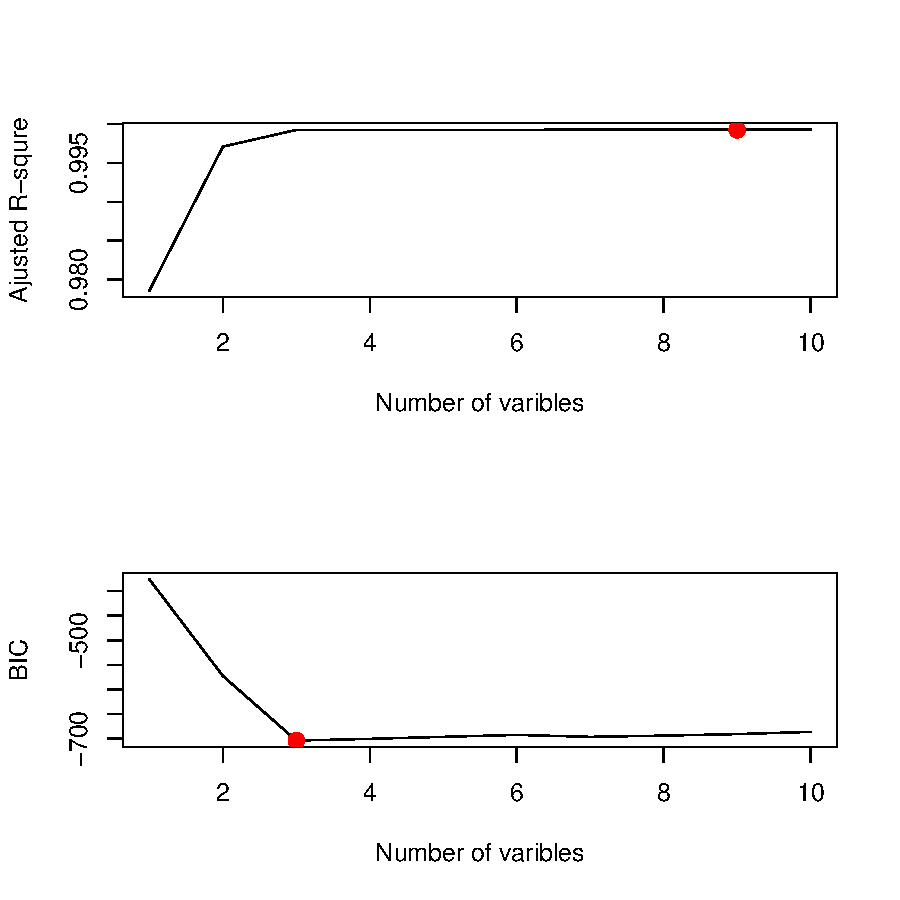
\includegraphics{modelselection-8cfig}
{\color{red}
\begin{enumerate}
\item Result of this problem is very UNSTABLE. Many facts will influence the final result of this problem:
\begin{itemize}
\item seed
\item if we set raw = T in ploy function
\item most importantly, how we choose beta.
\end{itemize}
Sometime, I get max adjr2 at index 7, sometimes at index 9 or 5.\\
But fortunately, BIC is relatively stable than adjr2, most of the time I get minimum BIC at index 3. Because BIC is more favorable to smaller number of variables.\\
\item As shown in the figure above, adjr2 reached its peak at index 3, and keep stable so on.
BIC reached its global minimum value at index 3, and this is the only minimum value.
\item The best predicted coef by BIC are close to its true value, as shown above.
\item However, the best predicted coef by adjr2 is not so, as shown above.
\end{enumerate}
}

\part{d}
\begin{Schunk}
\begin{Sinput}
> fit.fwd = regsubsets(y ~ poly(x, 10, raw = T), df, nvmax = 10, method = 'forward')
> fit.fwd.summary = summary(fit.fwd)
> # fit.fwd.summary
> which.max(fit.fwd.summary$adjr2)
\end{Sinput}
\begin{Soutput}
[1] 10
\end{Soutput}
\begin{Sinput}
> which.min(fit.fwd.summary$bic)
\end{Sinput}
\begin{Soutput}
[1] 3
\end{Soutput}
\begin{Sinput}
> par(mfrow = c(2, 1))
> plot(fit.fwd.summary$adjr2, xlab = 'Number of varibles', ylab = 'Ajusted R-squre', type = 'l')
> points(10, fit.fwd.summary$adjr2[3], col = 'red', cex = 2, pch = 20)
> plot(fit.fwd.summary$bic, xlab = 'Number of varibles', ylab = 'BIC', type = 'l')
> points(3, fit.fwd.summary$bic[3], col = 'red', cex = 2, pch = 20)
> coef(fit.fwd, 3)
\end{Sinput}
\begin{Soutput}
          (Intercept) poly(x, 10, raw = T)1 poly(x, 10, raw = T)2 
             1.965463              2.797556              3.962171 
poly(x, 10, raw = T)3 
            10.039204 
\end{Soutput}
\begin{Sinput}
> coef(fit.fwd, 10)
\end{Sinput}
\begin{Soutput}
           (Intercept)  poly(x, 10, raw = T)1  poly(x, 10, raw = T)2 
           2.169580713            2.659987801            1.451684521 
 poly(x, 10, raw = T)3  poly(x, 10, raw = T)4  poly(x, 10, raw = T)5 
          10.967635428            4.435167654           -0.730805121 
 poly(x, 10, raw = T)6  poly(x, 10, raw = T)7  poly(x, 10, raw = T)8 
          -2.516525214            0.154188775            0.541918393 
 poly(x, 10, raw = T)9 poly(x, 10, raw = T)10 
          -0.008679161           -0.038986881 
\end{Soutput}
\end{Schunk}
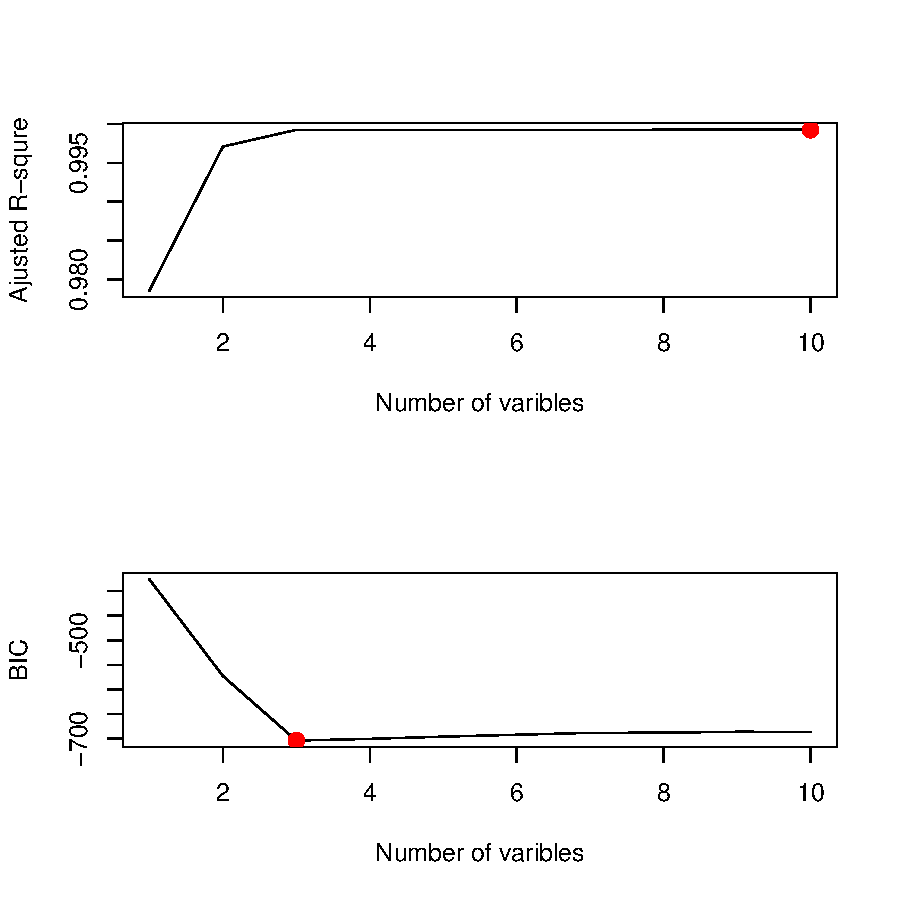
\includegraphics{modelselection-8df}
{\color{red}
\begin{enumerate}
\item Forward selection, basically, does not change too much from full selection.
\item This time adjr2 choose model at index 10. And BIC still choose model at index 3.
\item The coef of model at index 3 is still close to the true value.
\end{enumerate}
}
\begin{Schunk}
\begin{Sinput}
> fit.bwd = regsubsets(y ~ poly(x, 10, raw = T), df, nvmax = 10, method = 'backward')
> fit.bwd.summary = summary(fit.bwd)
> # fit.bwd.summary
> which.max(fit.bwd.summary$adjr2)
\end{Sinput}
\begin{Soutput}
[1] 9
\end{Soutput}
\begin{Sinput}
> which.min(fit.bwd.summary$bic)
\end{Sinput}
\begin{Soutput}
[1] 3
\end{Soutput}
\begin{Sinput}
> par(mfrow = c(2, 1))
> plot(fit.bwd.summary$adjr2, xlab = 'Number of varibles', ylab = 'Ajusted R-squre', type = 'l')
> points(9, fit.bwd.summary$adjr2[3], col = 'red', cex = 2, pch = 20)
> plot(fit.bwd.summary$bic, xlab = 'Number of varibles', ylab = 'BIC', type = 'l')
> points(3, fit.bwd.summary$bic[3], col = 'red', cex = 2, pch = 20)
> coef(fit.bwd, 3)
\end{Sinput}
\begin{Soutput}
          (Intercept) poly(x, 10, raw = T)1 poly(x, 10, raw = T)2 
             1.965463              2.797556              3.962171 
poly(x, 10, raw = T)3 
            10.039204 
\end{Soutput}
\begin{Sinput}
> coef(fit.fwd, 9)
\end{Sinput}
\begin{Soutput}
          (Intercept) poly(x, 10, raw = T)1 poly(x, 10, raw = T)2 
           2.00486068            2.18385089            3.35711858 
poly(x, 10, raw = T)3 poly(x, 10, raw = T)4 poly(x, 10, raw = T)5 
          12.56088616            1.03637630           -2.15396284 
poly(x, 10, raw = T)6 poly(x, 10, raw = T)7 poly(x, 10, raw = T)8 
          -0.45527056            0.60137906            0.05275883 
poly(x, 10, raw = T)9 
          -0.05228977 
\end{Soutput}
\end{Schunk}
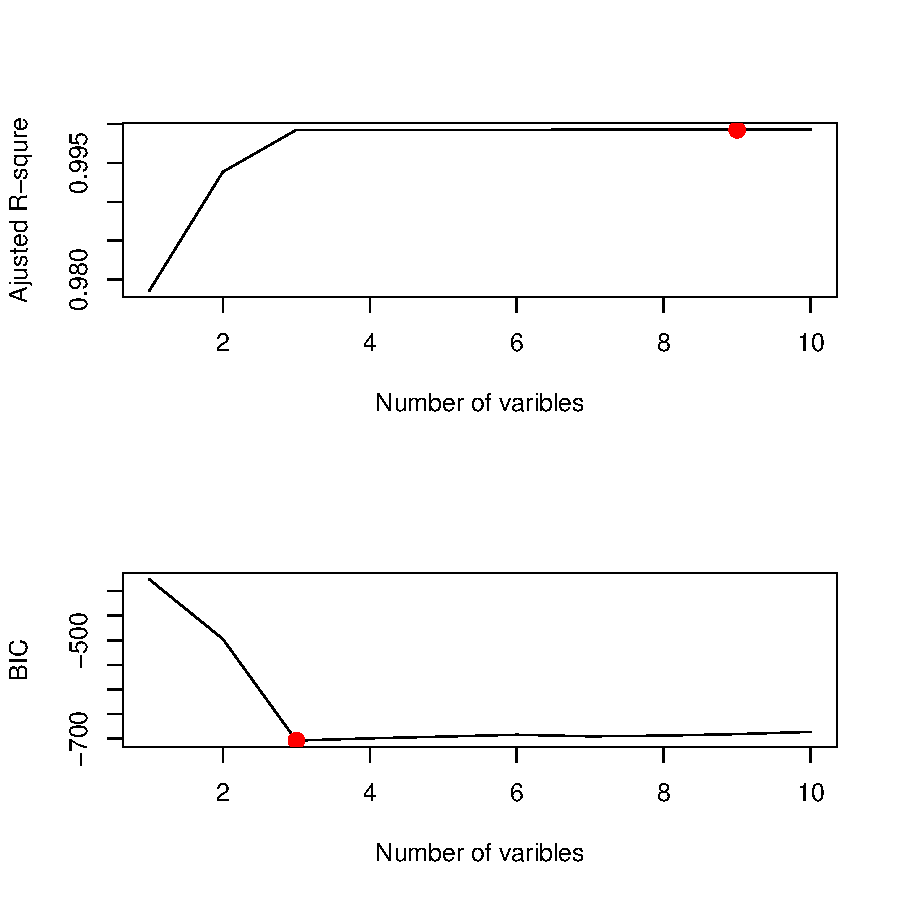
\includegraphics{modelselection-8db}
{\color{red}
\begin{enumerate}
\item Backward selection, also, does not change too much from full selection.
\item This time adjr2 choose model at index 9. And BIC still choose model at index 3.
\item The coef of model at index 3 is still close to the true value.
\end{enumerate}
}

\newpage

\question{11 - 1}{Predict per capita crime rate in Boston}
{\color{red}
\begin{enumerate}
\item Since Boston dataset only has 506 data points, we should use 10-folds cross validation to justify performance of model.\\
\item We use best selection to select candidate models, since there are only 13 predictors.\\
\end{enumerate}
}
\part{a \& b} best selection \& cross-validation\\
\begin{Schunk}
\begin{Sinput}
> library(MASS)
> bos = Boston
> attach(bos)
> predict.regsubsets = function(object, newdata, id, ...) {
+     form = as.formula(object$call[[2]])
+     mat = model.matrix(form, newdata)
+     coefi = coef(object, id = id)
+     xvars = names(coefi)
+     mat[, xvars] %*% coefi
+ }
> set.seed(0)
> k = 10
> pred.count = ncol(bos) - 1
> folds = sample(1:k, nrow(bos), replace = T)
> err.matrix = matrix(NA, k, pred.count)
> for (i in 1:k) {
+     fit.best = regsubsets(crim ~ ., bos[folds != i, ], nvmax = 13)
+     for (j in 1:pred.count) {
+ #         if (j == 9) {
+ #             print(coef(fit.best, j))
+ #         }
+         pred = predict(fit.best, bos[folds == i, ], id = j)
+         err.matrix[i, j] = mean((bos$crim[folds == i] - pred) ^ 2)
+     }
+ }
> mean.err = apply(err.matrix, 2, mean)
> which.min(mean.err)
\end{Sinput}
\begin{Soutput}
[1] 9
\end{Soutput}
\begin{Sinput}
> mean.err[which.min(mean.err)]
\end{Sinput}
\begin{Soutput}
[1] 39.09773
\end{Soutput}
\begin{Sinput}
> plot(mean.err, pch = 20, type = "b", col = 'red')
> fit.best = regsubsets(crim ~ ., bos, nvmax = 13)
> coef(fit.best, which.min(mean.err))
\end{Sinput}
\begin{Soutput}
  (Intercept)            zn         indus           nox           dis 
 19.124636156   0.042788127  -0.099385948 -10.466490364  -1.002597606 
          rad       ptratio         black         lstat          medv 
  0.539503547  -0.270835584  -0.008003761   0.117805932  -0.180593877 
\end{Soutput}
\end{Schunk}
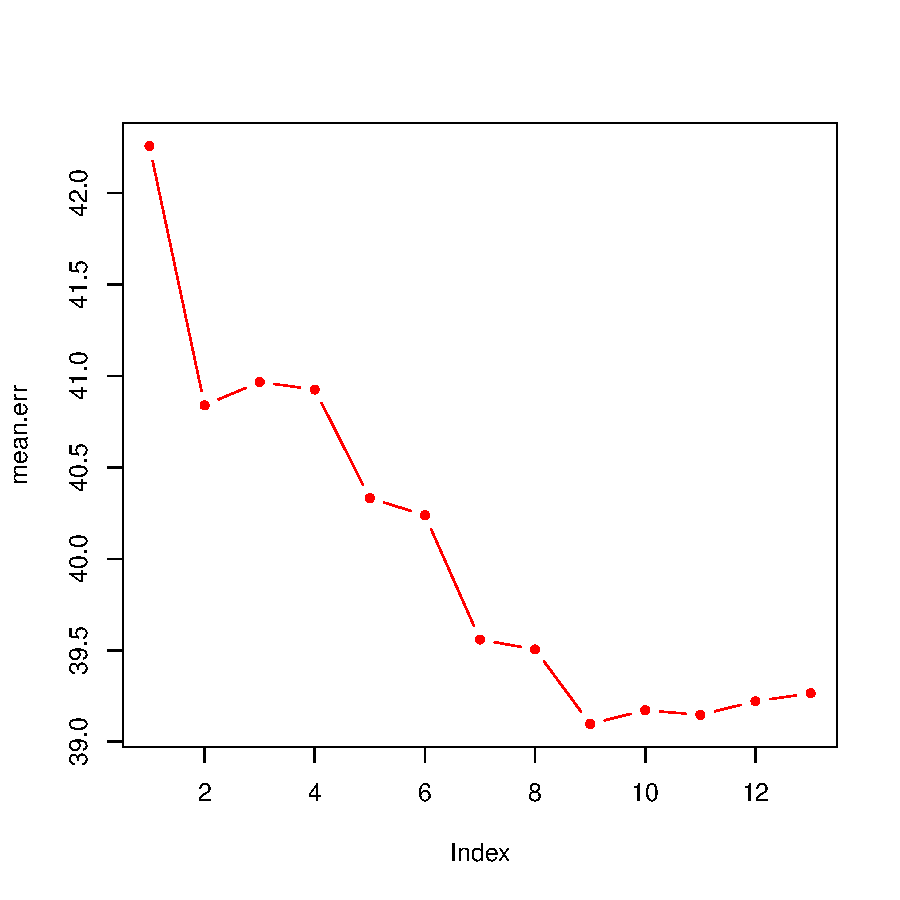
\includegraphics{modelselection-111a}

{\color{red}
\begin{enumerate}
\item Finally, it's easy to see that with 9 predictors we get the best perfromance on CV.
\item The best predictors and its coefficients are shown above.
\end{enumerate}
}

\part{c} analysis
{\color{red}
\begin{enumerate}
\item The finaly choosen model does not contain all of the features in the data sets.
\item Because as shown in the experiment above, model with 9 predictors has the lowest MSE on cross-validation sets.
\end{enumerate}
}

\newpage
\question{11 - 2}{Predict lsurv in Surgical}
{\color{red}
\begin{enumerate}
\item Since Surgical dataset only has 54 data points, I choose to use 5-folds cross validation to justify performance of model.\\
\item We use best selection to select candidate models, since there are only 8 predictors.\\
\item We only use log-survival time as reponse.
\end{enumerate}
}
\part{a \& b} best selection \& cross-validation\\
\begin{Schunk}
\begin{Sinput}
> rawdata = read.table('surgical.txt')
> surgical = rawdata[, -9]
> dimnames(surgical)[[2]] <- c('blood', 'prog', 'enz', 'liver',
+                       'age', 'female', 'modAlc', 'heavyAlc', 'lsurv')
> set.seed(0)
> k = 5
> pred.count = ncol(surgical) - 1
> folds = sample(1:k, nrow(surgical), replace = T)
> err.matrix = matrix(NA, k, pred.count)
> for (i in 1:k) {
+     fit.best = regsubsets(lsurv ~ ., surgical[folds != i, ], nvmax = 8)
+ 
+     for (j in 1:pred.count) {
+ #         if (j == 4) {
+ #             print(coef(fit.best, j))
+ #         }
+         pred = predict(fit.best, surgical[folds == i, ], id = j)
+         err.matrix[i, j] = mean((surgical$lsurv[folds == i] - pred) ^ 2)
+     }
+ }
> mean.err = apply(err.matrix, 2, mean)
> which.min(mean.err)
\end{Sinput}
\begin{Soutput}
[1] 4
\end{Soutput}
\begin{Sinput}
> mean.err[which.min(mean.err)]
\end{Sinput}
\begin{Soutput}
[1] 0.05218958
\end{Soutput}
\begin{Sinput}
> plot(mean.err, pch = 20, type = "b", col = 'red')
> fit.best = regsubsets(lsurv ~ ., surgical, nvmax = 8)
> coef(fit.best, which.min(mean.err))
\end{Sinput}
\begin{Soutput}
(Intercept)       blood        prog         enz    heavyAlc 
 3.85241856  0.07332263  0.01418507  0.01545270  0.35296762 
\end{Soutput}
\end{Schunk}
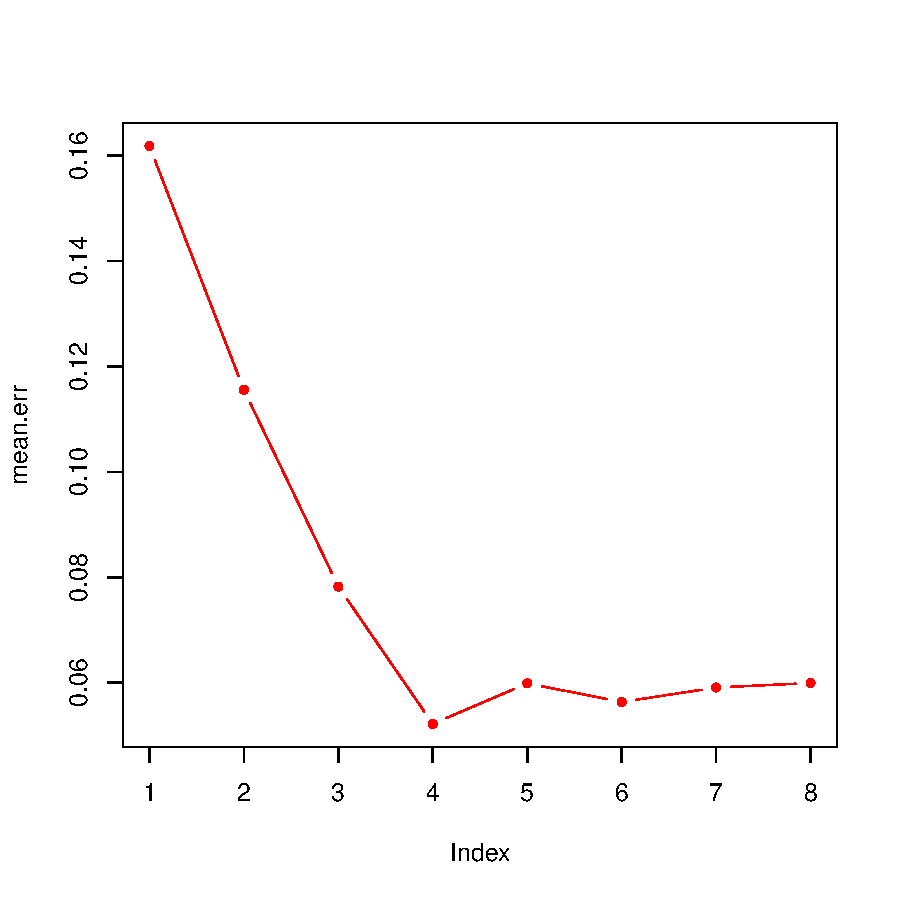
\includegraphics{modelselection-112a}
{\color{red}
\begin{enumerate}
\item Finally, it's easy to see that with 4 predictors we get the best perfromance on CV.
\item The best predictors and its coefficients are shown above.
\end{enumerate}
}

\part{c}
{\color{red}
\begin{enumerate}
\item Obviously my best model does not contain all the predictors. Since with 4 predictors my model get lowest MSE on CV.
\end{enumerate}
}

\end{document}
